\documentclass[a4paper,12pt]{article}
\usepackage[utf8]{inputenc}
\usepackage[spanish]{babel}
\usepackage{color}
\usepackage{parskip}
\usepackage{graphicx}
\usepackage{multirow}
\usepackage{listings}
\usepackage{vmargin}
\usepackage{datetime}
\newdate{date}{28}{09}{2017}
\graphicspath{ {imagenes/} }
\definecolor{mygreen}{rgb}{0,0.6,0}
\definecolor{lbcolor}{rgb}{0.9,0.9,0.9}
\usepackage{epstopdf}
\usepackage{float}


\setpapersize{A4}
\setmargins{2.5cm}       % margen izquierdo
{1.5cm}                        % margen superior
{16.5cm}                      % anchura del texto
{23.42cm}                    % altura del texto
{10pt}                           % altura de los encabezados
{1cm}                           % espacio entre el texto y los encabezados
{0pt}                             % altura del pie de página
{2cm}     

\lstset{
backgroundcolor=\color{lbcolor},
    tabsize=4,    
%   rulecolor=,
    language=[GNU]C++,
        basicstyle=\tiny,
        aboveskip={1.5\baselineskip},
        columns=fixed,
        showstringspaces=false,
        extendedchars=false,
        breaklines=true,
        prebreak = \raisebox{0ex}[0ex][0ex]{\ensuremath{\hookleftarrow}},
        frame=single,
        showtabs=false,
        showspaces=false,
        showstringspaces=false,
        identifierstyle=\ttfamily,
        keywordstyle=\color[rgb]{0,0,1},
        commentstyle=\color[rgb]{0.026,0.112,0.095},
        stringstyle=\color{red},
        numberstyle=\color[rgb]{0.205, 0.142, 0.73},
%        \lstdefinestyle{C++}{language=C++,style=numbers}’.
}


\begin{document}
\title{Práctica 3}
\author{
Christofer Fabián Chávez Carazas \\
\small{Universidad Nacional de San Agustín de Arequipa} \\
\small{Escuela Profesional de Ciencia de la Computación} \\
\small{Computación Centrada en Redes}
}
\date{\displaydate{date}}

\maketitle

\begin{large}
 \textbf{Actividades}
\end{large}

\begin{enumerate}
 \item \textbf{Cree la red 192.168.100.0 usando el software Packet Tracer, elija componentes genéricos.}
 \begin{figure}[H]
  \centering
  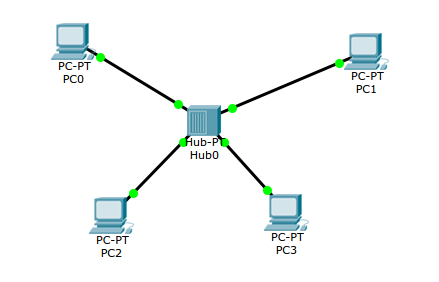
\includegraphics[scale = 0.5]{1.png}
  \caption{Red creada}
 \end{figure}
 \item \textbf{Indique la configuración de conectividad de cada PC (estado del puerto, tipo de conexión Ethernet según la velocidad-bandwidth, tipo de transmisión, dirección MAC, tipo y dirección IP, configuración IPv6)}
 \begin{figure}[H]
  \centering
  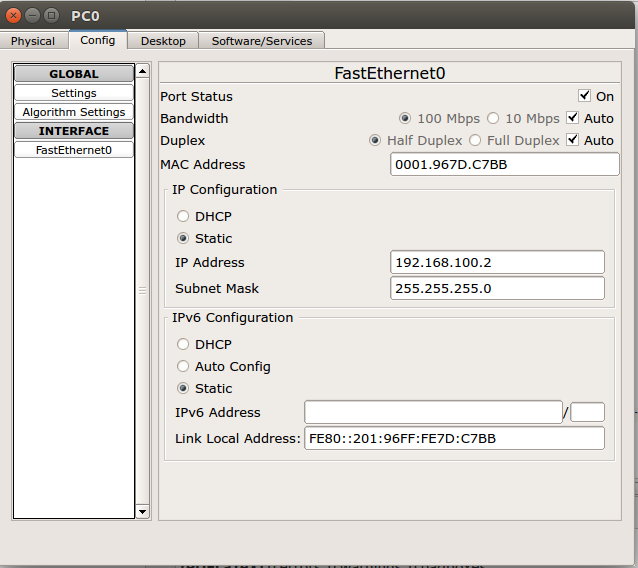
\includegraphics[scale = 0.5]{2.png}
  \caption{Configuración de la PC 0}
 \end{figure}
 \begin{figure}[H]
  \centering
  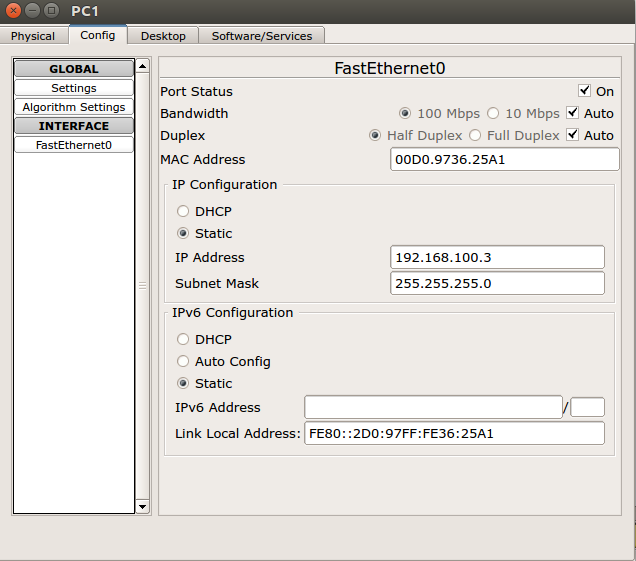
\includegraphics[scale = 0.5]{3.png}
  \caption{Configuración de la PC 1}
 \end{figure}
 \begin{figure}[H]
  \centering
  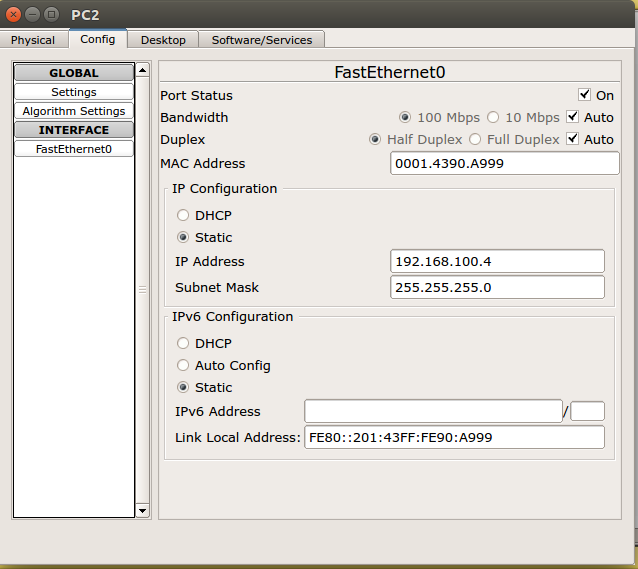
\includegraphics[scale = 0.5]{4.png}
  \caption{Configuración de la PC 2}
 \end{figure}
 \begin{figure}[H]
  \centering
  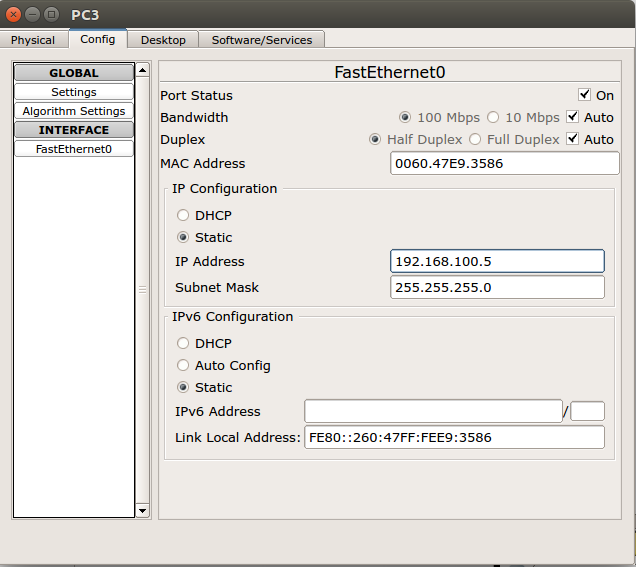
\includegraphics[scale = 0.5]{5.png}
  \caption{Configuración de la PC 3}
 \end{figure}
 \item \textbf{Identifique el tipo de puertos del hub, describa las características}
 \begin{figure}[H]
  \centering
  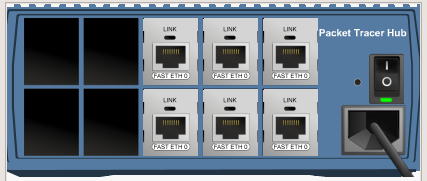
\includegraphics[scale = 0.5]{6.png}
  \caption{Puertos usados en el Hub}
 \end{figure}
 Los puertos usados en el Hub son los llamados PT-REPEATER-NM-1CFE. Según la descripción dada en el programa, éstos puertos
 proporcionan una interfaz \textit{Fast-Ethernet} para su uso con medios de cobre. Ideal para la amplia gama de aplicaciones LAN,
 los módulos de red \textit{Fast-Ethernet} admiten muchas características y estándares de interconexión.
 Los módulos de red de puerto único ofrecen autosensing 10/100BaseTX o 100BaseFX Ethernet. La versión TX(cobre) admite el despliegue de LAN virtual (VLAN).

 \item \textbf{Verifique que las conexiones estén activas (puntos verdes). Observe e identifique si han circulado paquetes de datos, si es así, describa la estructura de los mismo}
 \item \textbf{Envíe un mensaje simple (ping) de PC0 a PC1, que sucede. Identifique la secuencialidad y el tipo de PDU enviado en cada caso}
 \begin{figure}[H]
  \centering
  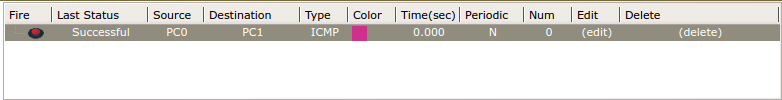
\includegraphics[scale = 0.5]{7.png}
  \caption{Mensaje PING enviado}
 \end{figure}
 \begin{figure}[H]
  \centering
  
\includegraphics[scale = 0.5]{8.png}
  \caption{PDU del mensaje}
 \end{figure}
  \begin{itemize}
   \item \textbf{¿Qué tipo de paquete es, describa la estructura del dato enviado a PC1 y la respuesta a PC0?} \\
   Los paquetes enviados son de tipo ICMP y la estructura se muestra en las figuras de abajo.
   \begin{figure}[H]
    \centering
    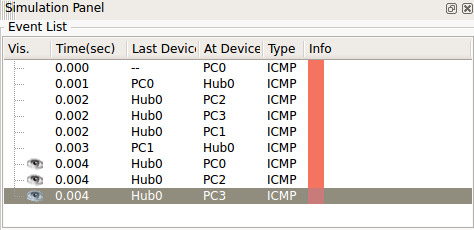
\includegraphics[scale = 0.5]{9.png}
    \caption{Paquetes enviados en todo el proceso}
   \end{figure}
   \begin{figure}[H]
    \centering
    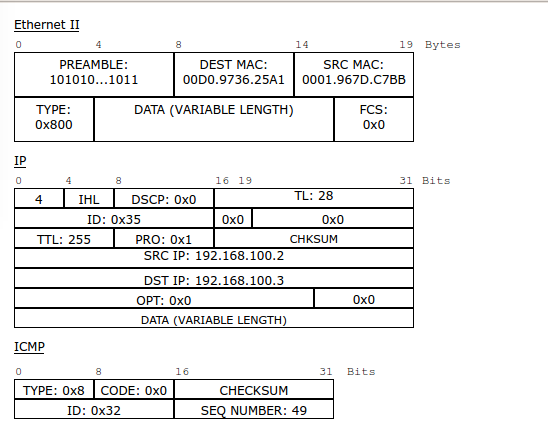
\includegraphics[scale = 0.5]{10.png}
    \caption{Estructura del dato enviado a PC1}
   \end{figure}
   \begin{figure}[H]
    \centering
    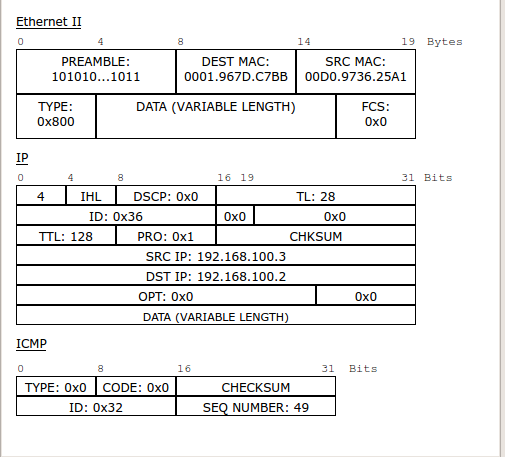
\includegraphics[scale = 0.5]{11.png}
    \caption{Estructura del dato enviado a PC0}
   \end{figure}
  \item \textbf{¿Por qué la propagación del hub involucra a todas las máquinas?} \\
  Porque la funcionalidad de un hub es esa. Lo que hace es recibir el paquete por uno de sus puertos, lo replica y lo envía a todos
  los demás puertos, excepto por el puerto por el que llegó el paquete.
  \end{itemize}
 
 \item \textbf{Repita configurando un mensaje como un ping entre PC2 y PC3}
 
 \begin{figure}[H]
  \centering
  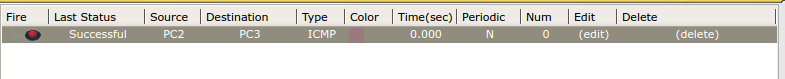
\includegraphics[scale = 0.5]{12.png}
  \caption{Mensaje enviado}
 \end{figure}
 
 \item \textbf{Modifique la dirección de PC3 a 192.168.100.2 explique qué es lo que sucede} \\
 No me deja poner la IP. Me manda un error diciendo que la IP ya está en uso en la red.
 \begin{figure}[H]
  \centering
  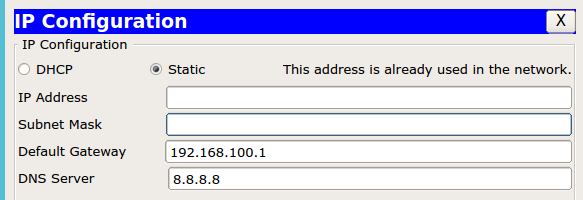
\includegraphics[scale = 0.5]{13.png}
  \caption{Mensaje de error}
 \end{figure}
 
 \item \textbf{Restaure la dirección de PC3, intente enviar dos PDUs simples de PC0 a PC1 y de PC2 a PC3, ¿qué sucede?} \\
 Hay una colisión en los paquetes.
 \begin{figure}[H]
  \centering
  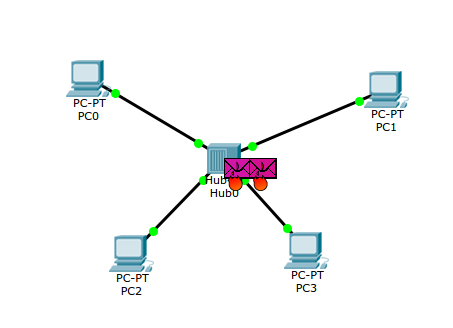
\includegraphics[scale = 0.5]{14.png}
  \caption{Momento de la colisión}
 \end{figure}
 
 \item \textbf{Cambie el hub por un switch repita 4.1.3 a 4.1.8, ¿cuál es la diferencia? explique. Observe la configuración del switch ¿en qué difiere de la configuración de un hub?, ¿por qué?}
 
 Una de las diferencias primordiales es que el switch sólo envía el paquete por el puerto de destino, ya no por todos los puertos como lo hace el hub.
 La otra mejora es que evita las colisiones. En el ejemplo donde con el hub había una colisión, el switch envió los paquetes sin problemas.
 Todo esto se debe a que el switch tiene procesador y memoria, lo que lo hace más inteligente que el hub. El switch guarda los dispositivos conectados
 a sus puertos.
\end{enumerate}


\begin{large}
 \textbf{Cuestionario}
\end{large}

\begin{enumerate}
 \item \textbf{Defina la diferencia entre un ICMP, un ARP y un STP} \par
 \begin{itemize}
  \item \textbf{El protocolo ICMP} \
  TCP utiliza este protocolo para el envío de mensajes de control y de error. Por ejemplo, ping se utiliza para ver si un ordenador está activo en la red.
  Los mensajes ICMP están dentro de datagramas IP (IP los trata igual que los demás datagramas). Es decir, dentro de los datos del datagrama, hay una cabecera del protocolo ICMP que indica una serie de parámetros como código de error, tipo de mensaje, etc., (como ya se ha dicho, IP no tiene constancia de que sea un datagrama especial).
  ICMP pueden enviar varios tipos de mensajes como por ejemplo, destino no alcanzable, control de congestión, redireccionamiento, tiempo excedido.
  \item \textbf{El protocolo ARP} \\
  Convierte las direcciones IP en direcciones físicas de la red. Cada host tiene una tabla para realizar dicha conversión. Cuando una dirección pedida no figura en la tabla, ARP genera una petición por toda la red. Si alguna máquina de la red recibe esa petición y corresponde con la suya propia, avisa al host que ha realizado la petición y este incluye la nueva dirección en su tabla de direcciones.
  \item \textbf{El protocolo STP} \\
  El objetivo del STP es mantener una red libre de bucles. Un camino libre de bucles se consigue cuando un dispositivo es capaz de reconocer un bucle en la topología y bloquear uno o más puertos redundantes.
  El protocolo STP explora constantemente la red, de forma que cualquier fallo o adición en un enlace, switch o bridge es detectado al instante. Cuando cambia la topología de red, el algoritmo de STP reconfigura los puertos del switch o el bridge para evitar una perdida total de la conectividad.
 \end{itemize}

 \item \textbf{Defina el concepto de PDU y ping}
 \begin{itemize}
  \item \textbf{PDU} \\
  Las unidades de protocolo de datos, también llamadas PDU, se utilizan para el intercambio de datos entre unidades disparejas, dentro de una capa del modelo OSI. Existen dos clases, PDU de datos; que contiene los datos del usuario principal,
  y PDU de control; que sirven para gobernar el comportamiento completo del protocolo en sus funciones de establecimiento y unión de la conexión, control de flujo, control de errores, etc.
  \item \textbf{Ping} \\
  PING es una herramienta, una utilidad de diagnosis utilizada en las redes informáticas para comprobar la comunicación entre nuestra máquina de origen y un destino remoto..
 \end{itemize}

 \item \textbf{¿Cuál es la diferencia entre un hub y un switch?, en cada caso identifique en que niveles de la torre OSI trabaja cada uno de ellos}
 \begin{itemize}
  \item \textbf{HUB} \\
  Un HUB simplemente une conexiones y no altera las tramas que le llega. Tiene las siguientes características:
  \begin{itemize}
   \item El HUB envía información a ordenadores que no están interesados.
   \item Este tráfico añadido genera más probabilidades de colisión.
   \item Un HUB funciona a la velocidad del dispositivo más lento de la red.
   \item Un HUB es barato.
   \item Un HUB casi no añade ningún retardo a los mensajes. 
   \item Los HUBs están situados en la capa 1, es decir la capa física ya que actúan como repetidores. 
  \end{itemize}
  \item \textbf{Switch} \\
  Un Switch tiene las siguientes características:
  \begin{itemize}
   \item El switch conoce los ordenadores que tiene conectados a cada uno de sus puertos.
   \item El switch almacena la trama antes de reenviarla.
   \item Un switch moderno también suele tener lo que se llama \textit{Auto-Negotation}, es decir, negocia con los dispositivos que se conectan a él la velocidad de funcionamiento.
   \item Velocidad de proceso: todo lo anterior requiere que el switch tenga un procesador.
   \item Los switchs se sitúan en la capa 2, es decir en la capa de Enlace de datos. 
  \end{itemize}
 \end{itemize}

 \item \textbf{Describa los tipos de datos manejados en cada nivel de la capa Ethernet, IP e ICMP, describa el encapsulamiento realizado}
 
 \begin{itemize}
  \item \textbf{Ethernet} \\
  Opera en la capa de enlace de datos y en la capa física. Tiene dos protocolos principales:
  \begin{itemize}
   \item LLC, que maneja la comunicación entre capas superiores e inferiores y Toma los datos del protocolo de red y agrega información de control para ayudar a entregar el paquete al destino.
   \item MAC, es el control de acceso al medio y encapsula los datos.
  \end{itemize}
  \begin{figure}[H]
   \centering
   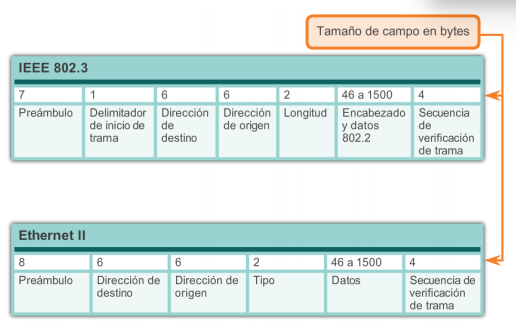
\includegraphics[scale = 0.5]{15.png}
   \caption{Formato de las tramas de Ethernet}
  \end{figure}
  \item \textbf{IP} \\
  Ofrece un servicio de envío de paquetes no orientado a conexión y no confirmado. Los paquetes del nivel IP se denominan datagramas, y son de longitud variable (hasta 65.536 bytes). Constan de dos partes:
  \begin{itemize}
   \item Campo de datos, donde se encapsulan las PDUs del nivel superior.
   \item Cabecera (denominada PCI en el modelo OSI). Contiene información necesaria para el encaminamiento de los paquetes. Su longitud puede variar entre 20 y 60 octetos
  \end{itemize}
  \begin{figure}[H]
   \centering
   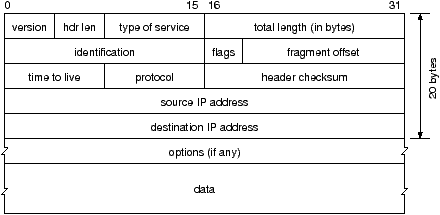
\includegraphics[scale = 0.6]{16.png}
   \caption{Formato del datagrama IP}
  \end{figure}
  \item \textbf{ICMP} \\
  El protocolo ICMP solamente informa de incidencias en la entrega de paquetes o de errores en la red en general, pero no toma decisión alguna al respecto. Esto es tarea de las capas superiores.
  Los mensajes ICMP se transmiten como datagramas IP normales, con el campo de cabecera ``protocolo'' con un valor 1, y comienzan con un campo de 8 bits que define el tipo de mensaje de que se trata. A continuación viene un campo código, de o bits, que a veces ofrece una descripción del error concreto que se ha producido y después un campo suma de control, de 16 bits, que incluye una suma de verificación de errores de transmisión. Tras estos campos viene el cuerpo del mensaje, determinado por el contenido del campo ``tipo''. Contienen además los 8 primeros bytes del datagrama que ocasionó el error.
  \begin{figure}[H]
   \centering
   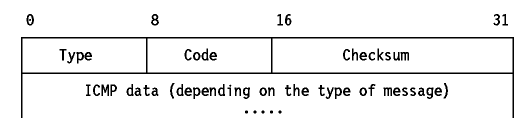
\includegraphics[scale = 0.6]{17.png}
   \caption{Formato del datagrama ICMP}
  \end{figure}
 \end{itemize}

 \item \textbf{¿Qué tipos de mensajes se pueden enviar?}
 
 \begin{itemize}
  \item Tipo 0: \textit{Echo Reply} (Respuesta de eco). Respuesta al mensaje Echo Request.
  \item Tipo 3: \textit{Destination Unreachable} (destino inaccesible). El destino no se puede alcanzar.
  \item Tipo 4: \textit{Source Quench} (Cadena de envío demasiado elevada). Enviado por un router cuando debe descartar paquetes de entrada, porque su cola de salida se ha llenado.
  \item Tipo 5: \textit{Redirect} (redireccionar). Enviado por un router a otro equipo para indicarle una mejor puerta de enlace para llegar al destino deseado.
  \item Tipo 8: \textit{Echo Request} (Petición de eco). Solicitud de eco, habitualmente generada por el comando ``ping''
  \item Tipo 9: \textit{Router Advertisement} (Aviso de router). Enviado por un router para dar a conocer un nuevo equipo a la red.
  \item Tipo 10: \textit{Router Solicitation} (Solicitud de Router). Enviado por un equipo o un router para pedir que otros routers envíen mensajes \textit{Router Advertisement}.
  \item Tipo 11: \textit{Time Exceded} (Tiempo sobrepasado). Enviado por un router cuando debe eliminar un paquete IP porque ha agotado su contador de saltos.
  \item Tipo 12: \textit{Parameter problem} (Problema de parámetros). Se usa como respuesta para errores que no tienen un mensaje ICMP específico.
  \item Tipo 13: \textit{Timestamp Request} (Petición de marca de tiempo). Solicita un paquete \textit{Timestamp Reply}.
  \item Tipo 17: \textit{Address Mask Request} (Petición de máscara de dirección). El router que recibe este mensaje debe responder con un Address Mask Reply.
  \item Tipo 18: \textit{Address Mask Reply} (Respuesta de máscara de dirección). Es una respuesta a la petición de tipo 17, con la que un router informa sobre la máscara correspondiente a la red por la que recibió la petición.
  \item Tipo 30: \textit{Traceroute Reply} (Respuesta de camino). Este mensaje lo debe enviar cada router que encamina o recibe un determinado paquete IP que contiene la opción Traceroute añadida en su cabecera.
 \end{itemize}

 \item \textbf{¿Cuál es el tamaño máximo de computadoras que se pueden interconectar usando el hub, el switch y el modem? ¿Por qué?} \par
 
 El número de computadoras que se pueden conectar a un determinado dispositivo depende del fabricante y el número de puertos que tenga.
 
 \begin{itemize}
  \item \textbf{Hub:} Puede tener 8, 16, 24 y 32 puertos.
  \item \textbf{Switch: } Puede tener 4, 8, 16, 24 y 48 puertos dependiendo del fabricante.
  \item \textbf{Modem: } Dependiendo del tipo de modem. Si es un modem inalámbrico, entonces el número máximo de conexiones
  depende del rango IP que tenga asignada la red.
 \end{itemize}

 
 \item \textbf{¿Qué función cumple un Gateway? ¿Por qué se le considera en la configuración? ¿Qué dirección IP recibe por convención?}
 
  Es el dispositivo que actúa de interfaz de conexión entre aparatos o dispositivos, y también posibilita compartir recursos entre dos o más computadoras. Su propósito es traducir la información del protocolo utilizado en una red inicial, al protocolo usado en la red de destino.
  Se le considera en la configuración porque dota a las máquinas conectadas al dispositivo de un acceso al exterior. Generalmente, una puerta de enlace recibe
  la primera IP de la red.
\end{enumerate}

\begin{large}
 \textbf{Conclusiones}
\end{large}

\begin{itemize}
 \item Actualmente no es muy recomendable usar hubs para conectar un número grande de computadoras, ya que, a más computadoras conectadas,
 más probabilidad hay de que ocurran colisiones entre los mensajes.
 \item Aunque el uso del switch es muy recomendable a la hora de sustituir un hub, se necesita configurar la red de forma óptima para obtener una mejor eficiencia.
 Para lograr esto se utiliza el subneteo.
\end{itemize}



\begin{thebibliography}{1}
 \bibitem{a}
 Jacinto Ruiz Catalán, ``Protocolos del nivel Internet: IP ICMP ARP RARP'', 2008.
 
 \bibitem{b}
 CISCO, ``Introducción y Configuración del Spanning Tree Protocol (STP) en los Switches Catalyst''
 
 \bibitem{c}
 Ausias March, ``Diferencias entre HUB y SWITCH''
 
 \bibitem{d}
 Aníbal Coto Cortés, ``Introducción a redes, Ethernet'', CISCO.

 \bibitem{e}
 Francisco A. y Jorge P., ``Manual de Práctica 2: Protocolo de Mensajes de Control de Internet (ICMP)'', 2009.
 
\end{thebibliography}



\end{document}

